\chapter{Sistemas operativos de software libre}
%\chapterauthor{Benito Federico, Filardo Juan, Simoncelli Fabricio, Ríos Julieta, Ulla Gonzalo}

Un sistema operativo libre es, como todo software libre, aquél que puede ser copiado, estudiado, modificado, utilizado libremente con cualquier fin y redistribuido con o sin cambios o mejoras.
En este capítulo presentaremos algunos sistemas operativos libres y su historia, ya que son fundamentales en el \emph{stack} de software libre.

\section{Historia de los SO derivados de Unix}

Los primeros sistemas operativos surgen en la década de 1950, pero la revolución es este campo ocurre durante los '60. Allí aparecen conceptos como sistemas multitareas, multiusuarios, multiprocesadores y de tiempo real. En esta década emerge Unix, base de la mayoría de los sistemas operativos libres actuales.

Unix fue desarrollado desde 1969 por Ritchie, Thompson y McIlroy en los laboratorios Bell de AT\&T. Es un sistema operativo portable, multitarea y multiusuario originalmente destinado a mainframes. Se caracteriza por poseer un núcleo monolítico y estar originalmente escrito en C (lenguaje a su vez creado por Ritchie).

Debido a que un fallo judicial antimonopolio impedía a la empresa de telecomunicaciones AT\&T comercializar software, Unix no fue comercializado inicialmente y se distribuía a las universidades con una licencia muy laxa. A partir de estas versiones de Unix varias universidades crearon sus propios sistemas operativos, el más exitoso y duradero es el sistema operativo libre BSD (por \emph{Berkeley Software Distribution})\footnote{BSD: \url{https://www.bsd.org/}} realizado en la Universidad de Californa en Berkeley. 

Por el problema de licencias mencionado y sus fortalezas técnicas, muchos sistemas operativos, libres o privativos, son variaciones de Unix. En la Fig.~\ref{figDerivUnix} vemos el árbol de sistemas operativos derivados de Unix, identificados por color según su esquema de licenciamiento: verde para fuentes abiertas, naranja pálido para los sistemas mixtos, con fuentes compartidas (pero no necesariamente abiertas o libres), y rosa para los sistemas privativos.

\begin{figure}[h!]
\centering
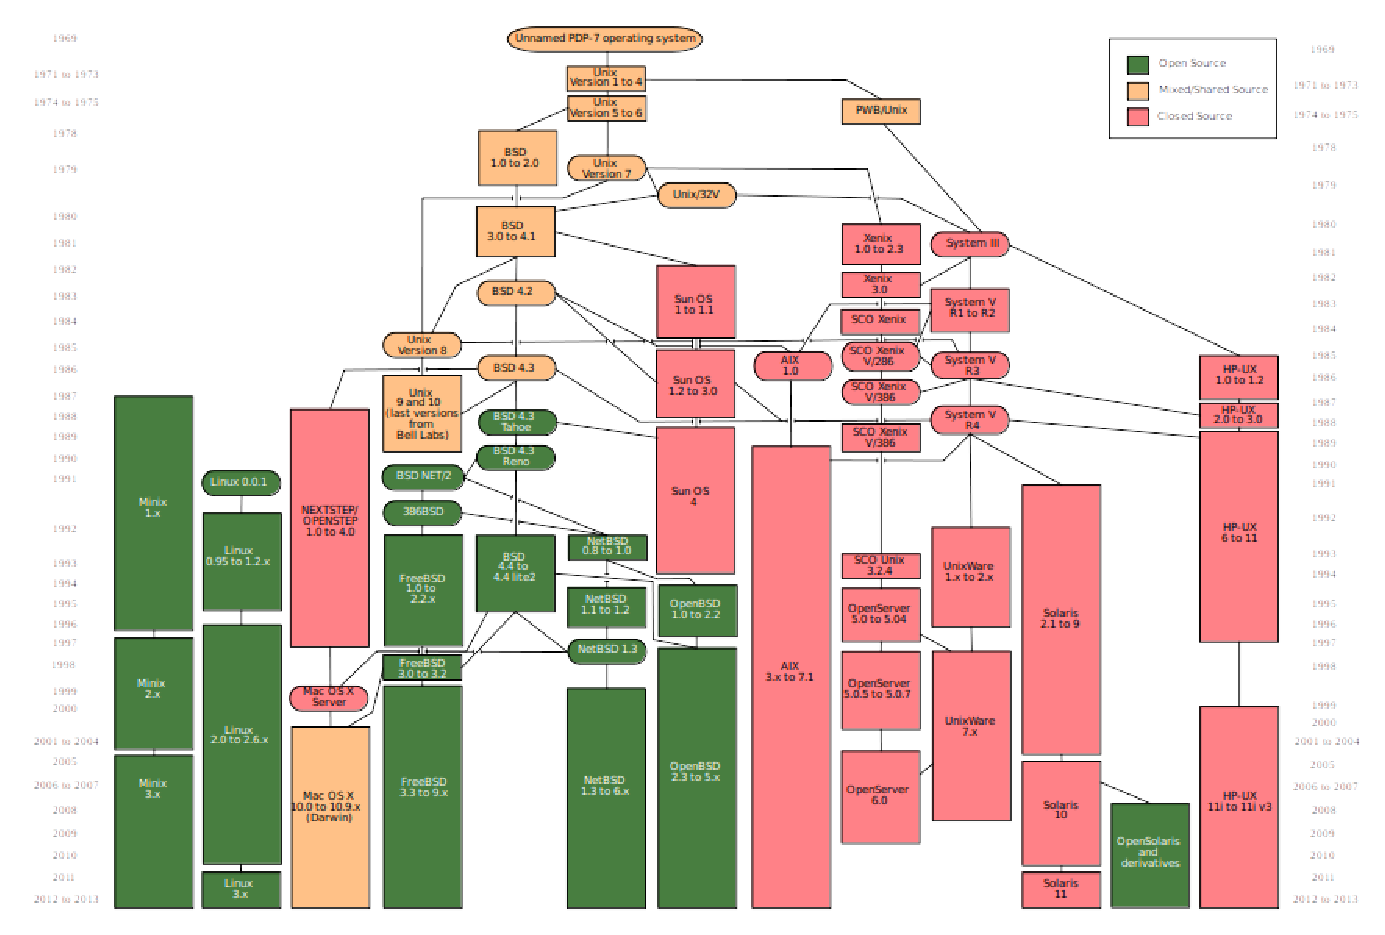
\includegraphics[scale=.5]{imagenes/arbolUnix.eps}
\caption{Sistemas operativos derivados de Unix.}
\label{figDerivUnix}
\end{figure}

Interesantemente, en las columnas de la izquierda podemos ver dos linajes derivados pero que no están conectados por una línea a Unix: Minix y Linux. La falta de conexión indica que, aunque derivados de Unix en el sentido de que siguen el estándar POSIX\footnote{Esto quiere decir que se comportan igual que Unix, respondiendo a los mismos comandos de la misma forma. Estándar POSIX: \url{https://es.wikipedia.org/wiki/POSIX}}, el código de estos sistemas operativos fue escrito desde cero. 

En el caso particular de Minix (llamado así por ser un MINI-uniX), este sistema operativo está basado en la tecnología de \emph{microkernel}, a diferencia de todos los otros sistemas de este árbol, que presentan un kernel monolítico. Otra particularidad de Minix es que durante mucho tiempo el código fuente impreso era parte del libro ``Sistemas Operativos: Diseño e Implementación''~\cite{tanenbaum87}, lo que hacía que el libro tuviera una longitud de 719 páginas. Ediciones posteriores eran acompañadas por versiones de Minix en diskettes o CD. Actualmente la versión 3 se puede obtener de un sitio web oficial\footnote{Minix 3: \url{http://www.minix3.org/}}.
	
\section{Distribuciones Linux}

Como se mencionó en el capítulo~\ref{capIntro}, los sistemas operativos libres más exitosos actualmente están basados en el núcleo (o \emph{kernel}) Linux. En vez de hablar de sistemas operativos diferentes, usualmente se los menciona como una ``distribución Linux'' (coloquialmente llamada \emph{distro}): una distribución es un sistema operativo basado en el núcleo Linux que incluye paquetes de software extra que le permiten satisfacer las necesidades de un grupo específico de usuarios. 

Una distribución Linux contiene típicamente el núcleo, herramientas y bibliotecas, software adicional, documentación, un sistema de ventanas, un administrador de ventanas y un entorno de escritorio. La mayor parte del software incluido es libreo o de fuentes abiertas y, por lo tanto, distribuido en binario compilado y en código fuente, permitiendo a sus usuarios modificar o compilar el código fuente original si lo desean. Muchas distribuciones incorporan software privativo, no disponible en forma de código fuente.

Si las distribuciones incluyen habitualmente las bibliotecas y herramientas del proyecto GNU, se la denomina GNU/Linux\footnote{La FSF (\textit{Free Software Foundation}) promueve el nombre de GNU/Linux para el sistema operativo en vez de solamente usar Linux, a fin de reconocer el aporte del proyecto GNU al sistema operativo, que no es sólo su núcleo o kernel, sino también controladores, aplicaciones de usuario y otros paquetes de software. Si bien el núcleo es el componente más grande del sistema, la sumatoria de todos los componentes GNU son mayores. Por su parte, quienes respaldan el uso del término Linux, dicen que es más corto y más fácil de nombrar. Además, argumentan que si se menciona uno de los colaboradores, se deberían mencionar todos.}). El sistema de ventanas más utilizado es X Window System, y los entornos de escritorio más comunes son: Gnome\footnote{Gnome: \url{https://www.gnome.org/}}, KDE\footnote{KDE: \url{https://kde.org/}}, XFCE\footnote{XFCE: \url{https://www.xfce.org/}} y Mate\footnote{Mate: \url{https://mate-desktop.org/}}.

Aunque son todas libres, existen distribuciones que están soportadas comercialmente, como Fedora\footnote{Fedora: \url{https://getfedora.org/}} (por Red Hat), openSUSE\footnote{openSUSE: \url{https://www.opensuse.org/}} (por Novell) o Ubuntu\footnote{Ubuntu: \url{https://ubuntu.com/}} (por Canonical), mientras que otras son mantenidas por una comunidad, como Debian\footnote{Debian: \url{https://www.debian.org/}} y Gentoo\footnote{Gentoo: \url{https://www.gentoo.org/}}. Incluso existen distribuciones que no están relacionadas con ninguna empresa o comunidad, sino con un único desarrollador, como es el caso de Slackware\footnote{Slackware: \url{http://www.slackware.com}} (también considerada como la distribución más antigua aún siendo mantenida).

Dado que seleccionando diferentes paquetes de software y empaquetándolos con sistemas automáticos se puede crear una nueva distribución a medida (de una empresa, un grupo o incluso una persona) en forma relativamente simple, es muy difícil llevar la cuenta de cuántas distribuciones Linux existen. El sitio DistroWatch\footnote{DistroWatch: \url{https://distrowatch.com/}} realiza un seguimiento de las distribuciones creadas y analiza si están activas o discontinuadas, además de publicar noticias sobre nuevas versiones, análisis de distribuciones y paquetes de software. Otra lista de distribuciones puede encontrarse en Wikipedia\footnote{\emph{List of Linux distributions} (la versión en español no es tan completa): \url{https://en.wikipedia.org/wiki/List_of_Linux_distributions}}.

\subsection{Clasificación de las distribuciones}

Como puede verse en la página \emph{List of Linux distributions} de Wikipedia, las distribuciones Linux se clasifican usualmente en base al sistema de gestión de paquetes que utilizan y a la distribución original de la cual derivan.

Cada paquete de software contiene una aplicación específica o un servicio (por ejemplo, una biblioteca para manejar el formato de imagen PNG, una colección de tipografías o un navegador web), la cual es generalmente distribuida en su versión compilada y su instalación (y desinstalación) es controlada por un ``sistema de gestión de paquetes''. Los paquetes elaborados para un sistema particular de paquetes contienen metadatos (tales como fecha de creación, descripción y dependencias) que son reconocidos por el sistema y utilizados para la búsqueda de paquetes correspondientes a las dependencias, por ejemplo. Algunos de los sistemas de paquetes más usados son:

\begin{itemize}
		\item RPM, creado por Red Hat y usado por un gran número de distribuciones de Linux, es el formato de paquetes del \emph{Linux Standard Base}.
		\item DEB, originalmente introducido por Debian, pero también utilizados por otras distribuciones muy conocidas, como Knoppix\footnote{Knoppix: \url{http://knoppix.net/}} y Ubuntu.
		\item .tgz, usado por Slackware, empaqueta el software usando tar y gzip. Pero no reporta los errores de dependencias encontrados, por lo que se utilizan algunas herramientas de más alto nivel para tratar con este formato: slapt-get, slackpkg y swaret. 
\end{itemize}

Entonces, la grilla de clasificación de distribuciones, considerando el sistema de paquetes que utilizan y la distribución original de la cual deriva es:

\begin{itemize}
\item RPM-based
  \begin{itemize}
  \item CentOS/RHEL-based
  \item  Fedora-based
  \item  openSUSE-based
  \item  urpmi-based
  \item  apt-rpm based
  \item  Independent RPM distributions
  \end{itemize}
\item DEB-based
  \begin{itemize}
  \item Debian-based
  \item MEPIS-based
  \item  Knoppix-based
  \item  Ubuntu-based
  \end{itemize}
\item Arch-based
\item Gentoo-based
\item Slackware-based
\end{itemize}


\subsection{¿Android es una distro Linux?}

Android, el sistema operativo más común en los teléfonos móviles, incluye un kernel Linux. Sin embargo, formalmente, existen diversas versiones de Android, en su mayoría desarrolladas para plataformas de hardware específicas, por lo que no pueden ser instaladas en cualquier computadora o teléfono móvil. Esta característica hace que no sean consideradas ``distribuciones''. Aunque existen algunos proyectos, tales como Android-x86\footnote{Android-x86: \url{https://www.android-x86.org/}}, que pueden ser instalados en hardware genérico, por lo que son usualmente consideradas como distribuciones.


%\subsection{Historia de las distribuciones Linux}
%Las distribuciones Linux comenzaron a surgir poco después de que el núcleo Linux fuera utilizado por otros programadores además de los creadores originales. Existía mayor interés en desarrollar un sistema operativo que en desarrollar aplicaciones, interfaces para los usuarios o un paquete de software conveniente.
%
%Entre las distribuciones más antiguas se incluían:
%
%\begin{itemize}
%	\item Dos discos denominados H J Lu's «Boot-root» con el núcleo y un mínimo de herramientas para utilizar.
%	\item MCC Interim Linux, que se podía descargar en un servidor público FTP de la Universidad de Manchester en febrero de 1992.
%	\item TAMU, creado por entusiastas de la Universidad de Texas A\&M al mismo tiempo que SLS.
%	\item SLS (Softlanding Linux System).
%	\item Yggdrasil Linux creó el primer CD-ROM de una distribución Linux.
%\end{itemize}
%
%SLS no estuvo bien mantenida; así pues, Patrick Volkerding lanzó una distribución basada en SLS a la que llamó Slackware; lanzada el 16 de julio de 1993. Esta es la distribución más antigua que está en desarrollo activo.
%Los usuarios vieron en Linux una alternativa a los sistemas operativos DOS, Microsoft Windows en la plataforma PC, Mac OS en Apple Macintosh y las versiones de uso bajo licencia (de pago) de UNIX. La mayoría de estos primeros usuarios se habían familiarizado con el entorno UNIX en sus trabajos o centros de estudios. Estos adoptaron GNU/Linux por su estabilidad, reducido (o nulo) coste y por la disponibilidad del código fuente del software incluido.
%Si bien, históricamente, Linux estuvo mejor posicionado en el mercado de los servidores, distribuciones centradas en la facilidad de instalación y uso, tales como Fedora, Mandriva, OpenSuSE, Knoppix y Ubuntu, entre otras, han logrado una mayor aceptación en el mercado doméstico.
%
%\subsection{¿GNU/Linux o Linux?}


%\subsection{Características de una distribución Linux}
%En general, las distribuciones Linux pueden ser:
%
%\begin{itemize}
%	\item Comerciales o no comerciales.
%	\item Ser completamente libres o incluir software privativo.
%	\item Diseñadas para uso en el hogar o en las empresas.
%	\item Diseñadas para servidores, escritorios o dispositivos empotrados.
%	\item Orientadas a usuarios regulares o usuarios avanzados.
%	\item De uso general o para dispositivos altamente especializados, como un cortafuegos, un enrutador o un clúster computacional.
%	\item Diseñadas e incluso certificadas para un hardware o arquitectura específicos.
%	\item Orientadas hacia grupos en específico, por ejemplo a través de la internacionalización y localización del lenguaje, o por la inclusión de varios paquetes para la producción musical o para computación científica.
%	\item Configuradas especialmente para ser más seguras, completas, portables o fáciles de usar.
%	\item Soportadas bajo distintos tipos de hardware.
%\end{itemize}
%
%La diversidad de las distribuciones Linux es debido a cuestiones técnicas, de organización y de puntos de vista diferentes entre usuarios y proveedores. El modo de licenciamiento del software libre permite que cualquier usuario con los conocimientos e interés suficiente pueda adaptar o diseñar una distribución de acuerdo a sus necesidades.


%\subsection{Distribuciones populares}
%
%Entre las distribuciones Linux más populares se incluyen:
%
%\begin{itemize}
%	\item \textit{Linux Mint} es una distribución de GNU/Linux comunitaria basada en Ubuntu que tiene por objeto proveer un sistema operativo moderno, elegante y confortable que sea tanto poderoso como fácil de usar.
%	\item \textit{Manjaro} es una distribución GNU/Linux, con Xfce, KDE o GNOME Shell como interfaz de usuario por defecto. Se trata básicamente de un sistema operativo libre para computadores personales y enfocado en la facilidad de uso. Está basado en Arch Linux y usa un modelo de desarrollo denominado rolling release.
%	\item \textit{Debian} es una distribución mantenida por una red de desarrolladores voluntarios con un gran compromiso por los principios del software libre.
%	\item \textit{Ubuntu} es un sistema operativo de código abierto. Está basada en la arquitectura de Debian. 
%	Está orientado al usuario promedio, con un fuerte enfoque en la facilidad de uso y en mejorar la experiencia del usuario.
%	\item \textit{Arch Linux} es una distribución basada en el principio KISS, con un sistema de desarrollo continuo entre cada versión (no es necesario volver a instalar todo el sistema para actualizarlo).
%	\item \textit{Canaima} es un proyecto socio-tecnológico abierto, construido de forma colaborativa, desarrollado en Venezuela y basado en Debian.
%	\item \textit{CentOS} es una distribución creada a partir del mismo código del sistema Red Hat pero mantenida por una comunidad de desarrolladores voluntarios.
%	\item \textit{Chakra project} es una popular distribución para escritorio, inicialmente basada en Arch Linux, actualmente se encuentra en un desarrollo independiente.
%	\item \textit{Elementary OS} es una distribución Linux basada en Ubuntu. Orientada a una interfaz amigable y muy estética.
%	\item \textit{Fedora} es una distribución lanzada por Red Hat para la comunidad.
%	\item \textit{Gentoo}, es una distribución orientada a usuarios avanzados.
%	\item \textit{Knoppix} fue la primera distribución live en correr completamente desde un medio extraíble. Está basada en Debian.
%	\item \textit{Kubuntu} es la versión en KDE de Ubuntu.
%\end{itemize}
%
%\subsection{Distribuciones especializadas}
%Otras distribuciones se especializan en grupos específicos:
%
%\begin{itemize}
%	\item \textit{Huayra}, distribución Educativa, desarrollada por el estado Argentino, desde el Anses para el Programa Conectar Igualdad. Está basada en Debian Jessie con entorno de escritorio MATE.
%	\item \textit{64 Studio}, una distribución basada en Debian diseñada para la edición multimedia.
%	\item \textit{ABC GNU/Linux}, distribución para la construcción de clusters Beowulf desarrollado por Iker Castaños Chavarri, Universidad del País Vasco.
%	\item \textit{Kali Linux}, distribución basada en Debian y especializada en seguridad de red.
%	\item \textit{BackTrack}, distribución basada en Ubuntu y especializada en seguridad de red.
%	\item \textit{WiFiSlax}, distribución basada en Slackware y especializada en seguridad de red.
%	\item \textit{Wifiway}, distribución basada en Ubuntu y especializada en seguridad de red.
%	\item \textit{Debian Med}, es una distro orientada a la práctica médica y a la investigación bio-médica.
%	\item \textit{Tails}, es una distribución especializada en la privacidad. Sólo corre live cd.
%\end{itemize}


\section{BSD (\emph{Berkeley Software Distribution})}

\emph{Berkeley Software Distribution} (BSD)\footnote{BSD: \url{https://www.bsd.org/}} es una familia de sistemas operativos derivada del sistema Unix. Tal como dijimos previamente, nació a partir de los aportes realizados a Unix por docentes e investigadores de la Universidad de California en Berkeley (Estados Unidos). Debido a la prohibición que pesaba sobre la empresa de telecomunicaciones AT\&T de vender sistemas informáticos, en los primeros años del sistema Unix sus creadores, los Laboratorios Bell de AT\&T, distribuyeron copias en varias universidades y les autorizaron a utilizar el código fuente y adaptarlo a sus necesidades.

Durante los años 1970 y 1980 Berkeley utilizó el sistema para sus investigaciones en materia de sistemas operativos. Cuando AT\&T retiró el permiso de uso a la universidad por motivos comerciales, la universidad promovió la creación de una versión inspirada en el sistema Unix utilizando los aportes que ellos habían realizado, permitiendo luego su distribución con fines académicos y finalmente eliminando toda restricción respecto a su copia, distribución o modificación. Tales derechos se plasmaron en la licencia del sistema BSD, la cual no incluye la obligatoriedad de que los trabajos derivados sean distribuidos con la misma licencia (es decir, es una licencia ``permisiva'').

Esto posibilita, además, que su código fuente sea incorporado legalmente en software no libre. Así, otros sistemas operativos, tanto libres como propietarios, han incorporado código BSD. Por ejemplo, Microsoft Windows utiliza código derivado de BSD en su implementación de TCP/IP.
 
\subsection{Versiones de BSD}

Las diferentes versiones (o \emph{flavors} en inglés\footnote{La traducción de \emph{flavors} al idioma español es ``sabores''.}) del sistema operativo BSD fueron aportando componentes importantes a la familia Unix de sistemas operativos y también generaron una rama muy importante de sistemas derivados que aún seguimos utilizando. 

\begin{itemize}
	\item BSD 1 era un añadido a la sexta edición de Unix. Más que un sistema operativo completo era un Unix con el agregado de un compilador Pascal y un editor de texto.
	\item BSD 2 fue lanzada en 1978 e incluía dos nuevos programas que perduran en los sistemas Unix hasta hoy en día: el editor de textos \texttt{vi} y el \emph{shell} del lenguaje C.
	\item BSD 3 fue la primera distribución considerada como un sistema operativo completo. Era una modificación del novedoso Unix 7.
	\item BSD 4.3 incorporó la licencia permisiva libre BSD.
\end{itemize}

A partir de este linaje de versiones se derivaron varios sistemas operativos relevantes:

\begin{itemize}
	\item SunOS\footnote{SunOS: \url{https://es.wikipedia.org/wiki/SunOS}} de la empresa Sun Microsystems. Utilizado en los poderosos servidores que esa compañía manufacturaba hasta principios de los '90.
	\item Variaciones de BSD para distintos públicos o usos: FreeBSD\footnote{FreeBSD: \url{https://www.freebsd.org/es/}} para servicios web, NetBSD\footnote{NetBSD: \url{https://netbsd.org/}} para portabilidad, TrueOS (orignalmente llamado PC-BSD) para computadoras personales\footnote{TrueOS o PC-BSD: \url{https://es.wikipedia.org/wiki/TrueOS}} y OpenBSD\footnote{OpenBSD: \url{https://www.openbsd.org/}} basado en la seguridad.
	\item NeXTSTEP\footnote{NeXTSTEP: \url{https://es.wikipedia.org/wiki/NEXTSTEP}} de la empresa NeXT de Steve Jobs, que derivó a su vez en Mac OS X\cite{michan10}.
\end{itemize}

 
\section{ReactOS}

ReactOS\footnote{ReactOS: \url{https://reactos.org/}} es un sistema operativo de código abierto que trata de emular la arquitectura de Windows NT. Este sistema operativo comenzó a desarrollarse en 1995 con el nombre de FreeWin95 pues era un clon de Windows 95. A partir de 1998 cambió su nombre a ReactOS y ha continuado con la incorporación gradual y permanente de características de las últimas versiones de Windows. Está principalmente escrito en C, con algunos elementos, tales como ReactOS Explorer y la pila del sonido, escritos en C++. Las licencias de este sistema operativo son: GNU GPL, LGPL y BSD.

El objetivo de ReactOS es el de proveer un sistema operativo el cual sea compatible a nivel binario con Windows y brindar una interfaz familiar para los y las usuarias. De este modo, podrán usar fácilmente este sistema como una alternativa libre a Windows, sin tener que cambiar el software al que están acostumbrados.

%\subsection{Versiones importantes}
%
%\begin{itemize}
%	\item La primera versión del sistema, con interfaz gráfica de usuario funcional, salió en enero de 2004.
%	\item En febrero de 2017 salió la última versión (0.4.4) que incluye: Soporte inicial de pila de impresión, correcciones menores de fuentes, mejoras y correcciones de errores.
%	\item La próxima versión del sistema va a ser la 0.5 y va a ser considerada Beta. No se sabe cuando sale, pero si lo que va a incluir: Soporte de escritura para NTFS, soporte para drivers WDM (Windows Driver Model), impresoras y DirectX.
%	\item A marzo de 2018 es considerado como software alfa, que, si bien posee características incompletas, muchas aplicaciones de Windows ya funcionan y por lo tanto es recomendado por desarrolladores solamente para propósitos de evaluación y prueba.
%\end{itemize}

%\subsection{Chrome OS}
%
%Es el sistema operativo de Google basado en la nube de kernel linux con licencia BSD y de c\'odigo abierto. Se dice ``basado en la nube'' ya que puede prescindir de disco duro y toda la informaci\'on del usuario queda en servidores de Google, el inicio del mismo es sumamente r\'apido con un tiempo de booting de 8 segundos y solo funciona bajo microprocesadores x86 o ARM.
%
%\subsection{Un poco de historia}
%
%\begin{itemize}
%     \item En Julio de 2009 Google anuncia el Sistema Operativo.
%     \item En Noviembre 2009 se libera el código fuente bajo licencia BSD y a mayo del 2010 ya hab\'ia 1.000.000 de descargas, el proyecto es llamado Chromium OS. 
%     \item En Diciembre 2010 se crea un programa piloto el cual google envia a usuarios de Estados Unidos chromebooks llamadas CR-48 sin costo alguno con el fin de obtener feedback de usuarios.
%     \item En Mayo 2011 se realiza el lanzamiento de chromebooks fabricados por socios de Google, ellos son Acer y Samsung.
%\end{itemize}
%
%%\newpage
%\subsection{Carater\'isticas}
%
%La interfaz gr\'afica de Chrome OS es minimalista aproxim\'andose a Mac OS y Windows siendo sus principales competidores, la principal idea es contar con un Sistema Operativo con escritorio orientado hacia internet y Google lo considera una extensión natural del navegador Chrome.
%\\
%\\
%Otras Caracter\'isticas:
%
%\begin{itemize}
%     \item Soporta la ejecuci\'on solamente de aplicaciones Web.
%     \item Requisitos mínimos de hardware: RAM: 2GB, Disco duro: 6GB.
%     \item Interfaz Gr\'afica del navegador de Chrome.
%	 \item Corre bajo hardware específico y preinstalado en Chromebooks.
%\end{itemize}
%
%\section{Chromium OS}
%
%Es el código abierto de la versión de desarrollo Google Chrome OS. Fue construido sobre la base de un núcleo Linux, en un entorno Ubuntu 10.04, utilizando el gestor de paquetes oficial de la distribución Linux Gentoo, Portage. De este modo, se dice que es un híbrido entre Ubuntu y Gentoo, dado que se basa en ambas distribuciones.
%Las licencias de este sistema operativo son: BSD y otras.
%Por otro lado, la arquitectura de Chromium OS está dividida en tres capas: el firmware, el navegador web y el gestor de ventanas.
%\\
%El código fuente fue descargado mas de 1.000.000 de veces a mayo del 2010 y, en ese momento, surge una versión popular llamada Chromium OS Flow creada por Liam McLoughlin. Esto hizo más interesante al sistema operativo, ya que incorpora compilaciones desde memoria USB y también la posibilidad de ejecutar aplicaciones desarrolladas en Java. Muchos ingenieros de Google quedaron sorprendidos ya que, dichas características, no habían sido imaginadas ni implementadas por ellos y, lo más interesante aún, es que Liam McLoughlin solo tenía 17 años.
%\\
%\\
%Para convertirse en colaborador los siguientes links pueden ser de utilidad:
%\begin{itemize}
%     \item Sitio del proyecto: http://dev.chromium.org/chromium-os
%     \item C\'odigo fuente: git clone https://chromium.googlesource.com/chromiumos
%\end{itemize}

%\newpage

\section{Sistemas operativos para móviles}

Además de los servidores, las computadoras personales y las portátiles, el dispositivo computacional más difundido hoy en el mundo son los teléfonos móviles o ``inteligentes'' (de \emph{smartphone}, en inglés). Como ya se mencionó, el sistema operativo más utilizado en estos dispositivos es Android, el cual está basado en el núcleo Linux. Sin embargo, Android no es software libre y no existen a la fecha sistemas operativos libres para teléfonos móviles que tenga una porción de mercado mínimamente relevante.

El éxito de Android se debió a que fue el sistema operativo seleccionado por la \emph{Open Handset Alliance} (OHA)\footnote{OHA: \url{https://www.openhandsetalliance.com/}}, la cual es una alianza comercial de 86 compañías que desarrolla estándares para dispositivos móviles. Algunos de sus miembros son Google, HTC, Dell, Intel, Motorola, Qualcomm, Texas Instruments, Samsung, LG, T-Mobile, Nvidia y AMD.

%Al mismo tiempo que se anunciaba la formación de la Open Handset Alliance el 5 de noviembre de 2007, la OHA presentó Android, una plataforma de código libre para teléfonos móviles basada en el núcleo operativo Linux. Una beta del SDK fue lanzada para desarrolladores el 12 de noviembre de 2007. Basado en una licencia de código libre, compite contra otras plataformas móviles propietarias de Apple, Microsoft, Nokia, Palm, BlackBerry (compañía) y Bada.

No faltaron intentos de producir sistemas operativos libres para teléfonos móviles, entre los que recordamos a Firefox OS\footnote{Firefox OS: \url{https://support.mozilla.org/es/products/firefox-os}}, Tizen\footnote{Tizen: \url{https://www.tizen.org/}} y Ubuntu Touch\footnote{Ubuntu Touch: \url{https://ubuntu-touch.io/es/}}, pero ninguno de ellos fueron comercialmente exitosos.


%Un sistema operativo móvil comprende un conjunto de programas de bajo nivel que permiten la abstracción de las peculiaridades del hardware específico del teléfono móvil y proveen servicios a las aplicaciones móviles que se ejecutan sobre él. Al igual que las PCs que utilizan Windows o Linux o Mac, los dispositivos moviles tienen sus sistemas operativos como Android, IOS Windows Phone, entre otros.
%
%\subsection{Sistemas Operativos Mobile Open Source}
%
%\subsubsection{Firefox OS}
%Firefox OS es un sistema operativo móvil, basado en HTML5 con núcleo Linux, de código abierto para varias plataformas. Fue desarrollado por Mozilla Corporation bajo el apoyo de otras empresas, como Telefónica, y una gran comunidad de voluntarios de todo el mundo. Este sistema fue enfocado especialmente en los dispositivos móviles, smartphones y tabletas, incluidos los de gama baja. Estuvo diseñado para permitir a las aplicaciones HTML5 comunicarse directamente con el hardware del dispositivo usando JavaScript y Open Web APIs. También ha sido mostrado en otros dispositivos como Raspberry Pi y televisores.
%En febrero de 2013 Mozilla anunció planes para el lanzamiento mundial de Firefox OS. Mozilla comunicó en rueda de prensa antes del inicio del Mobile World Congress en Barcelona, que la primera ola de dispositivos con Firefox OS estaría disponible en Brasil,Colombia, Hungría, México, Montenegro, Polonia, Serbia, España y Venezuela. Firefox también anunció que LG Electronics, ZTE, Huawei y TCL Corporation se habían comprometido a la fabricación de dispositivos con Firefox OS.
%A finales de 2015, Mozilla Corporation da por concluido el desarrollo del sistema Firefox OS para móviles bajo el argumento de que el proyecto no logró el objetivo de ofrecer a los usuarios la mejor experiencia posible. Los principales obstáculos encontrados al desarrollo del sistema fueron de tipo comercial.
%
%\subsubsection{Ubuntu Touch}
%Ubuntu Touch es un sistema operativo móvil basado en Linux. Fue desarrollado por Canonical. Presentado el 2 de enero de 2013 al público mediante un anuncio en la web de Ubuntu, culmina el proceso de Canonical de desarrollar una interfaz que pueda utilizarse en ordenadores de sobremesa, portátiles, netbooks, tablets y teléfonos inteligentes. Esta interfaz, Unity, se compone, a grandes rasgos, de un dock a la izquierda, una especie de panelesen la parte superior y un sistema de búsqueda que emplea "lentes".
%Ubuntu Touch se caracteriza por ser un sistema diseñado para plataformas móviles. 
%Sus características más destacadas son:
%\begin{itemize}
%	 \item Pantalla de inicio sin sistema de bloqueo/desbloqueo (que funciona con un nuevo sistema de gestos, y que se aprovecha para mostrar notificaciones).
% 	 \item Ubuntu Touch incluye como aplicaciones centrales de medios sociales y medios de comunicación (por ejemplo, aplicaciones de Facebook, YouTube, y un lector de RSS ). Las aplicaciones estándar, tales como una calculadora, un cliente de correo electrónico, un despertador, un gestor de archivos, e incluso un terminal están incluidos también. En este momento doce o más aplicaciones principales se están desarrollando.
% 	 \item Integración con Ubuntu One.
%\end{itemize}
%
%
%\subsubsection{Tizen}
%Tizen es un sistema operativo móvil basado en Linux, patrocinado por Linux Foundation y la Fundación LiMo. Tizen se construye a partir de la plataforma Linux de Samsung (Samsung Linux Platform - SLP) una implementación de referencia integrada en LiMo. El 1 enero de 2012, la fundación LiMo es renombrada como Asociación Tizen dirigida por un Consejo de Administración de Samsung, Intel, Huawei, Fujitsu, NEC, Panasonic, KT Corporation, Sprint Corporation, SK Telecom, Orange, NTT DoCoMo y Vodafone. La Asociación Tizen trabaja en estrecha colaboración con la Fundación Linux, que apoya el proyecto de código abierto Tizen.
%
%Las interfaces de desarrollo de Tizen están basadas en HTML5 y otros estándares web y fueron diseñadas para su uso en tabletas, netbooks, teléfonos inteligentes, televisores inteligentes y sistemas integrados de información y entretenimiento.
%
%El 22 de julio de 2013 fue liberada la versión 2.2. Tizen será compatible con las aplicaciones actuales de Android. Los desarrolladores han hecho hincapié en que HTML5 no es la única plataforma disponible y también se han integrado las bibliotecas Enlightenment Foundation Libraries en el sistema operativo.
%
%Aunque originalmente fue presentado como un sistema operativo de código abierto, Tizen 2 ha complicado su modelo de licencias. Su SDK está construido sobre componentes de código abierto, pero el SDK completo ha sido publicado bajo una licencia de Samsung de código no abierto.
%
%El sistema operativo en sí mismo está compuesto de muchos componentes de código abierto. Una serie de componentes internos desarrollados por Samsung, como la animación del arranque y las aplicaciones de calendario, gestor de tareas y de reproductor de música son, sin embargo, publicados bajo la licencia Flora License la cual, probablemente, es incompatible con los requisitos de la Open Source Initiative.
%
%%\newpage
%\subsubsection{Android}
%Android es un sistema operativo basado en el núcleo Linux. Fue diseñado principalmente para dispositivos móviles con pantalla táctil, como teléfonos inteligentes, tablets y también para relojes inteligentes, televisores y automóviles. 
%Inicialmente fue desarrollado por Android Inc., empresa que Google respaldó económicamente y más tarde, en 2005, compró. Android fue presentado en 2007 junto la fundación del Open Handset Alliance (un consorcio de compañías de hardware, software y telecomunicaciones) para avanzar en los estándares abiertos de los dispositivos móviles. El primer móvil con el sistema operativo Android fue el HTC Dream y se vendió en octubre de 2008. Los dispositivos de Android venden más que las ventas combinadas de Windows Phone e IOS.
%Android está basado en el kernel de Linux, el cual es distribuido bajo licencia GNU GPL v2.0, mientras que las librerías nativas y el framework de este sistema operativo posee licencia Apache v2.0. Esto permite que la gran mayoría de aplicaciones que corren en Android posean licencias privativas.
%\\
%\\
%{\bf  Open Handset Alliance}
%\\
%La Open Handset Alliance (OHA) es una alianza comercial de 84 compañías que se dedica a desarrollar estándares abiertos para dispositivos móviles. Algunos de sus miembros son Google, HTC, Dell, Intel, Motorola, Qualcomm, Texas Instruments, Samsung, LG, T-Mobile, Nvidia y Wind River Systems.
%Al mismo tiempo que se anunciaba la formación de la Open Handset Alliance el 5 de noviembre de 2007, la OHA presentó Android, una plataforma de código libre para teléfonos móviles basada en el núcleo operativo Linux. Una beta del SDK fue lanzada para desarrolladores el 12 de noviembre de 2007. Basado en una licencia de código libre, compite contra otras plataformas móviles propietarias de Apple, Microsoft, Nokia, Palm, BlackBerry (compañía) y Bada.
%El primer teléfono comercialmente disponible con Android fue el T-Mobile G1 (también conocido como HTC Dream). Fue aprobado por la FCC el 18 de agosto de 2008, y salió a la venta el 22 de octubre.
%\\
%\\
%{\bf ASOP}
%\\
%La versión básica de Android es conocida como Android Open Source Project (AOSP). La cual está disponible desde la página de Android.
%\\
%\\
%{\bf CyanogenMod}
%\\
%Poco después de la introducción del terminal HTC Dream en septiembre de 2008, la comunidad de desarrolladores Android encontró un método para obtener permisos de superusuario (root) en el subsistema Linux de Android (procedimiento conocido como 'rooteado' del dispositivo). Este descubrimiento, combinado con la naturaleza de código abierto de Android, permitió modificar los firmwares originales y reinstalarlos en el teléfono a voluntad. 
%CyanogenMod, comúnmente abreviado y conocido como CM, fue un sistema operativo de código abierto discontinuado para teléfonos móviles y tabletas basado principalmente en el popular sistema operativo Android. Fue desarrollado como software libre y de código abierto basado en las versiones oficiales de Android desarrolladas por Google donde se le agrega código propio y de terceros. Siguió un modelo de desarrollo rolling release.
%Ofreció varias características, herramientas y aplicaciones adicionales que no se encuentran en las versiones oficiales basadas en Android suministradas por los fabricantes originales de Teléfonos móviles. Algunas de estas características son el soporte nativo de temas, soporte para códec de audio FLAC, una gran cantidad de nombres de puntos de acceso, un cliente de OpenVPN, una aplicación de control de permisos por aplicación llamado Privacy Guard, soporte para tethering mediante Wi-Fi, Bluetooth o USB, overclocking de CPU y otras mejoras de desempeño, acceso de superusuario, entre otras.
%CyanogenMod aseguraba que sus modificaciones mejoran el rendimiento y la fiabilidad frente a las versiones oficiales del software. De acuerdo con sus desarrolladores y debido a su modelo de desarrollo de código abierto (lo cual hace que cualquier individuo pueda verificar la autenticidad de esta afirmación), CyanogenMod no contiene spyware o bloatware.
%Los servicios de CyanogenMod dejaron de estar operativos a partir del 31 de diciembre de 2016, siendo discontinuado y sustituido en su lugar por el proyecto abierto LineageOS.
%
%%\section{Herramientas de Desarrollo Open Source}
%%Una gran cantidad de herramientas han sido creadas orientadas principalmente al desarrollo de aplicaciones multiplataforma tanto como para sistemas operativos open source como para propietarios. Estas herramientas en su gran mayoria son Open Source 
%%Entre ellas podemos encontrar:
%%\begin{itemize}
%%	 \item React Native
%% 	 \item Ionic
%% 	 \item Cordova y sus Librerias
%%\end{itemize}